\section{Analysis of deadlock problem}\label{sec:analysis}

\subsection{Deadlock problem in RDMA DCNs}\label{subsec:deadlock_problem}

Once a loop occurs in a network, packets of some flows will be caught in the loop and traverse the same links multiple times until they are dropped due to Time-to-Live (TTL) expiration. Apart from causing packet drops, loops will also waste some link bandwidth as well as increase the end-to-end delay for the flows traversing some link(s) in the loop (but not caught by the loop).

\begin{figure}[t]
\centering
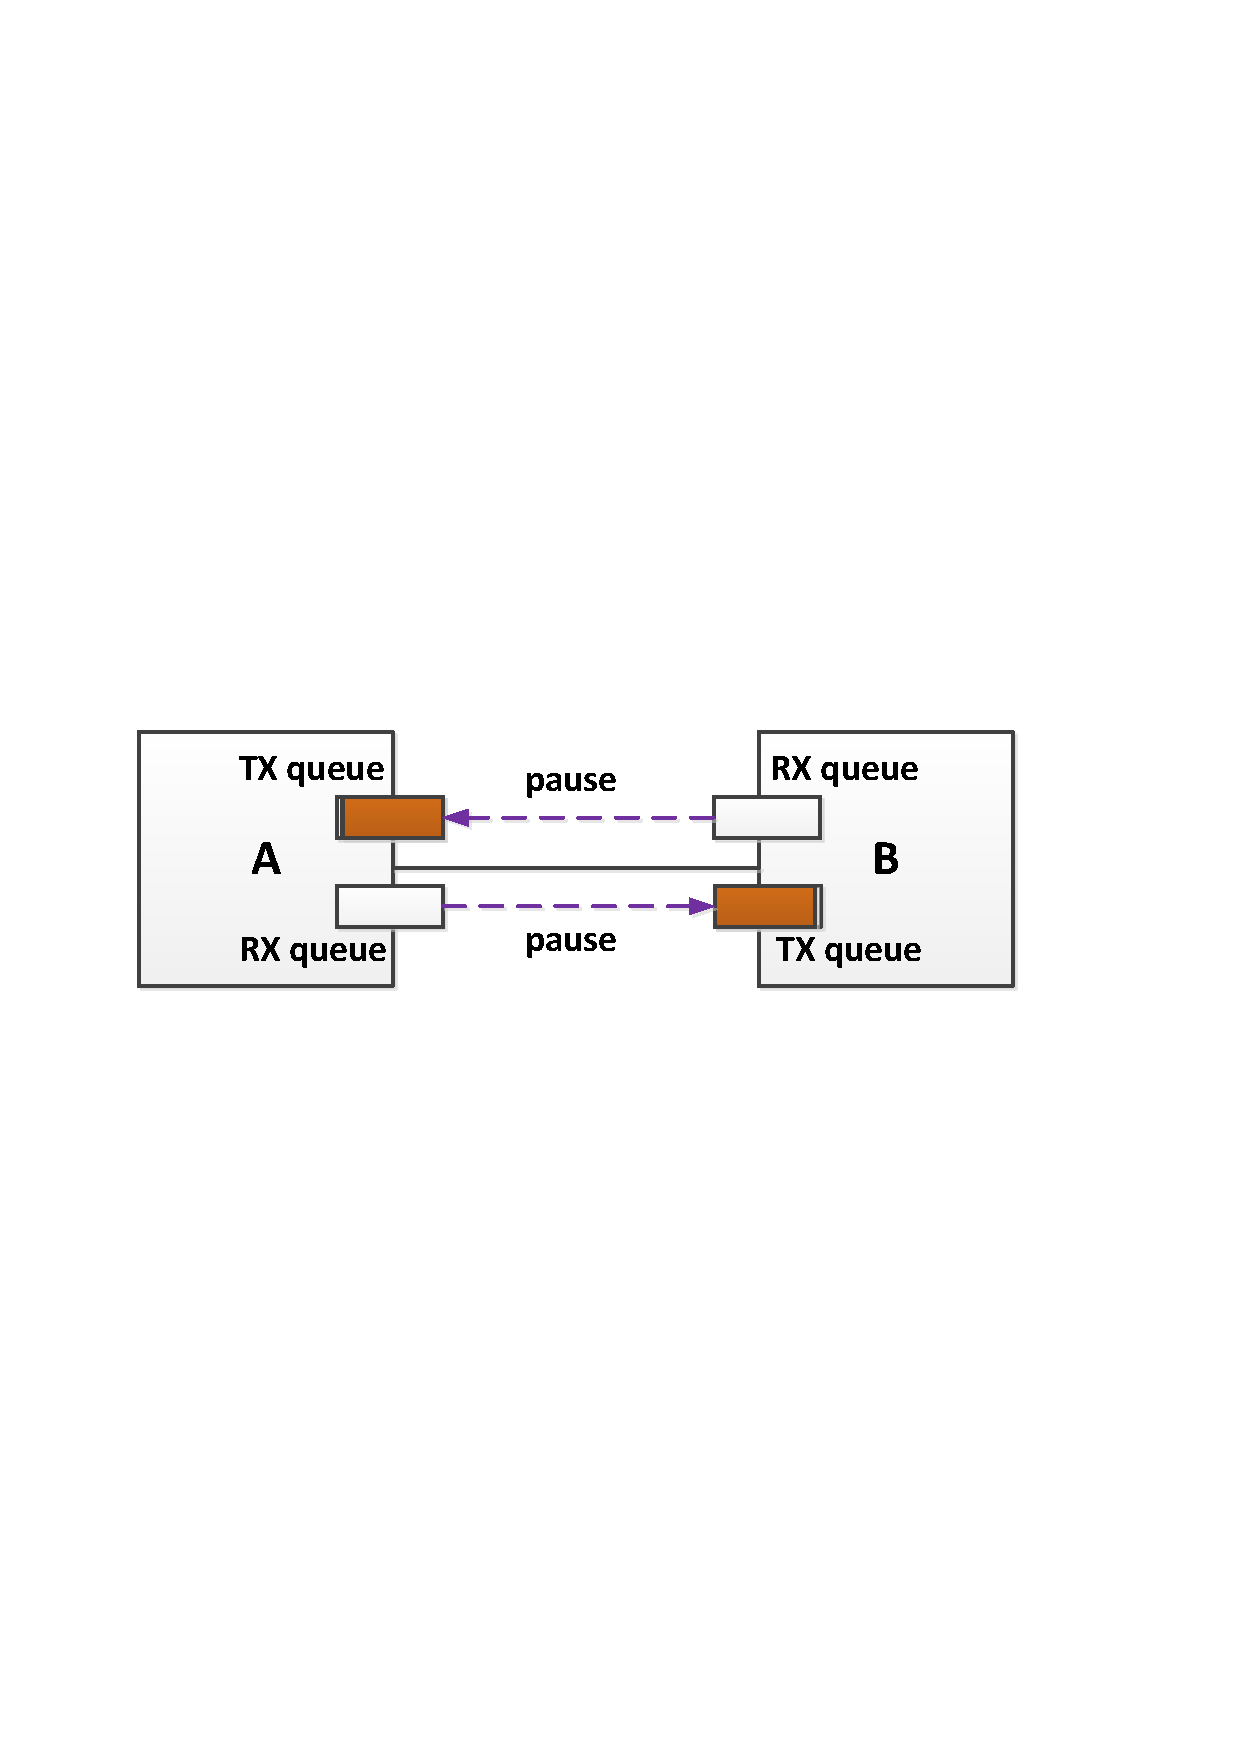
\includegraphics[width=0.45\textwidth,center]{figs/deadlock_example.pdf}
\caption[Optional caption for list of figures]{An example of loop induced deadlock: there is a loop between switch A and switch B. Both TX queues (egress queues) are paused by PFC as no buffer are available at both switches to accommodate more packets.}
\label{fig:loop_deadlock}
\end{figure}

In a lossy network, the impact of a loop is not fatal and can be completely eliminated as long as the loop is removed from the network. In contrast, in a lossless network, if packets enter a loop faster than they get dropped in the loop due to TTL expiration, packets will occupy the buffer of all the switches in the loop, and then a deadlock is created. When a deadlock occurs, each switch in the loop is paused by its downstream switch, and at the same time pauses its upstream switch due to the lack of available buffer to accept more packets. Once such a circular buffer dependency is created, the deadlock condition will hold persistently even after the loop is eliminated. 

 Under deadlock condition, no packets can move along the links in the loop, and more and more devices outside the loop will be paused due to the cascade effect of PFC. If a deadlock is created in the core of the network, it is very likely to bring the whole data center into a deadlock state.

A simple deadlock example is shown in Fig.~\ref{fig:loop_deadlock}. In this example, there is a routing loop between switch A and switch B. Packets enter this loop at a sufficient large rate and soon occupy all the available buffer of both switches. Then Both TX queues (egress queues) will be paused by PFC PAUSE frames and a deadlock is created. As we can see, this deadlock cannot be resolved by eliminating the routing loop as packets are already queued in the TX queues and can never reach the next-hop switch to escape from the loop.

\subsection{Sufficient condition for deadlock creation}\label{subsec:deadlock_condition}

In this part, we analyze the sufficient condition to create a deadlock when there is a loop in the network.  

At first, we consider the maximum packet drain rate in a loop regarding TTL expiration. Let $n$ the number of switches in a loop, $B$ be the link bandwidth and $k_{TTL}$ be the TTL value of packets before they enter the loop. Each time a packet traverses one switch, its TTL value will be reduced by 1.

The maximum packet drain rate is achieved when no switch is paused by PFC PAUSE frame and each switch is sending packets to its next-hop in the loop at the rate of $B$. So the maximum packet drain rate $r^{max}_d$ is equal to $nB/k_{TTL}$. here $nB$ can be viewed as the maximum packet ``flowing" rate in the loop, while $1/k_{TTL}$ captures the information that a packet will be dropped after it has traversed $k_{TTL}$ hops of switches in the loop.

Let $r_{in}$ be the injection rate of packets into the loop. One sufficient condition to create a deadlock in a lossless network is that: there is a loop 
in the network, and condition $r_{in} > r^{max}_d$ holds for a sufficient long period until a circular buffer dependency is created in the loop.

\begin{figure}[t]
\centering
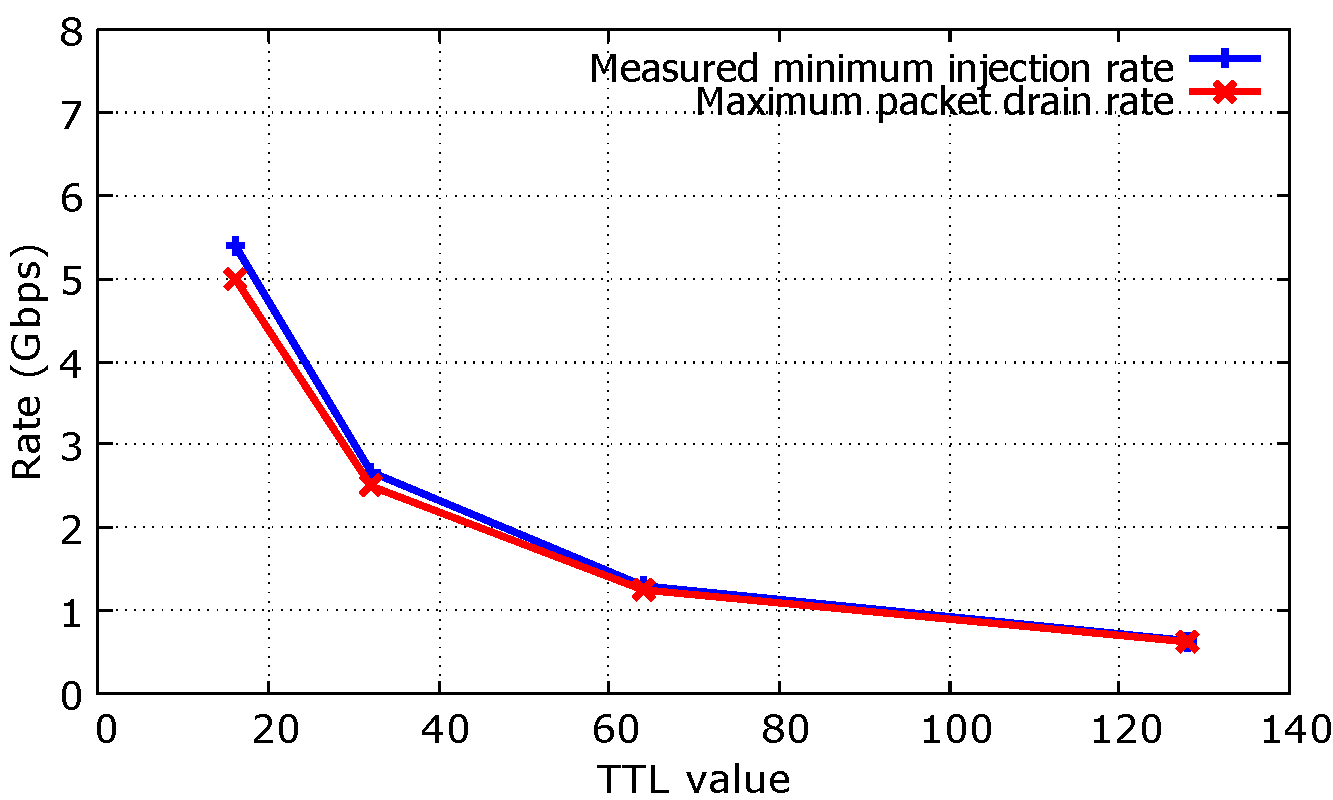
\includegraphics[width=0.5\textwidth,center]{figs/r_and_rdrain.pdf}
\caption[Optional caption for list of figures]{Measurement of the minimum injection rate to create a deadlock. Both switches in the loop are Arista 7050QX32.}
\label{fig:mrate_measurement}
\end{figure}

To verify our analysis above, we manually configure a loop between two 40Gbps switches, and measure the minimum packet injection rate that can create a deadlock. The result is shown in Fig.~\ref{fig:mrate_measurement}. As we can see, the measured minimum packet injection rate is just slightly larger than the maximum packet drain rate which is computed according to $nB/k_{TTL}$. This observation holds when TTL is set to different values. 

Another observation from the figure is that, setting smaller TTL can help to prevent deadlock but its benefit is limited. As shown in the figure, when TTL is set to 16 which is already a very small value, the minimum injection rate is only about 6Gbps.

\subsection{Analysis of the time to create a deadlock}\label{subsec:deadlock_condition}

In this part, we analyze and measure the time to create a deadlock when the sufficient condition for deadlock creation is already met. Deadlock creation time is related to three factors: \textbf{packet injection rate $r_{in}$}, \textbf{packet drain rate $r_{d}$} and \textbf{PFC threshold $t_{PFC}$}. 

$t_{PFC}$ determines the minimum bytes of packets needed to be ``trapped" in the loop to create a deadlock, while $r_{in} - r_{d}$ can be viewed as the packet increase rate.

%Packet injection rate is determined by the instant traffic demand of applications running in the data center. A larger injection rate requires less time to create a deadlock.
%
%As discussed above, the maximum packet drain rate will be a fixed value once $n$, $B$ and $k_{TTL}$ is determined. We find that packet drain rate will decrease significantly after packets are queued in the loop because it will take a packet much longer time to get dropped in the loop when there is queuing delay.

Most modern commodity switches use a dynamic $\alpha$ algorithm to determine the value of PFC threshold: Let $\alpha$ be a parameter with the range from 0 to 1, $m$ be the total switch buffer size and $m^\prime$ be the amount of buffer currently occupied. For a given $\alpha$, the value of $t_{PFC}$ is dynamically computed according to the following equation $ t_{PFC} = \alpha(m - m^\prime)$. During runtime, once the queue length of an ingress queue exceeds the instant $t_{PFC}$, a PAUSE frame will be sent to its upstream device. Note that a PAUSE frame will take some time to arrive an upstream device and take effect. To avoid packet loss due to this delay, some buffer headroom must be reserved for each ingress queue, and hence the value of $m$ in the equation is usually slightly smaller than the total switch buffer size.

%
 
 
 %Most modern commodity switches share memory buffer among all ports. In order to better utilize the available shared buffer in a timely fashion, instead of setting a fixed PFC threshold,
%A PAUSE frame will take some time to arrive an upstream device and take effect. To avoid packet loss due to this propagation delay, we must reserve enough
%buffer headroom for each ingress queue to accommodate packets a switch may receive before a PAUSE frame finally takes effect. Let $\Delta m$ be the total amount of reserved buffer headroom. The $m$ in the above equation should be modified to be $m - \Delta m$.
%Switches and NICs will track the value of $m^\prime$ and update the value of $t_{PFC}$ during runtime. 

%A smaller $\alpha$ value can lead to a shorter creation time of deadlock.  This is because a smaller $\alpha$ value means a smaller PFC threshold, while a smaller PFC threshold requires less packets to trigger a switch queue to send PAUSE frames to stop its upstream neighbors.

In the next, we measure the time to create a deadlock when setting different $\alpha$ and TTL values.


\begin{figure}[t]
\centering
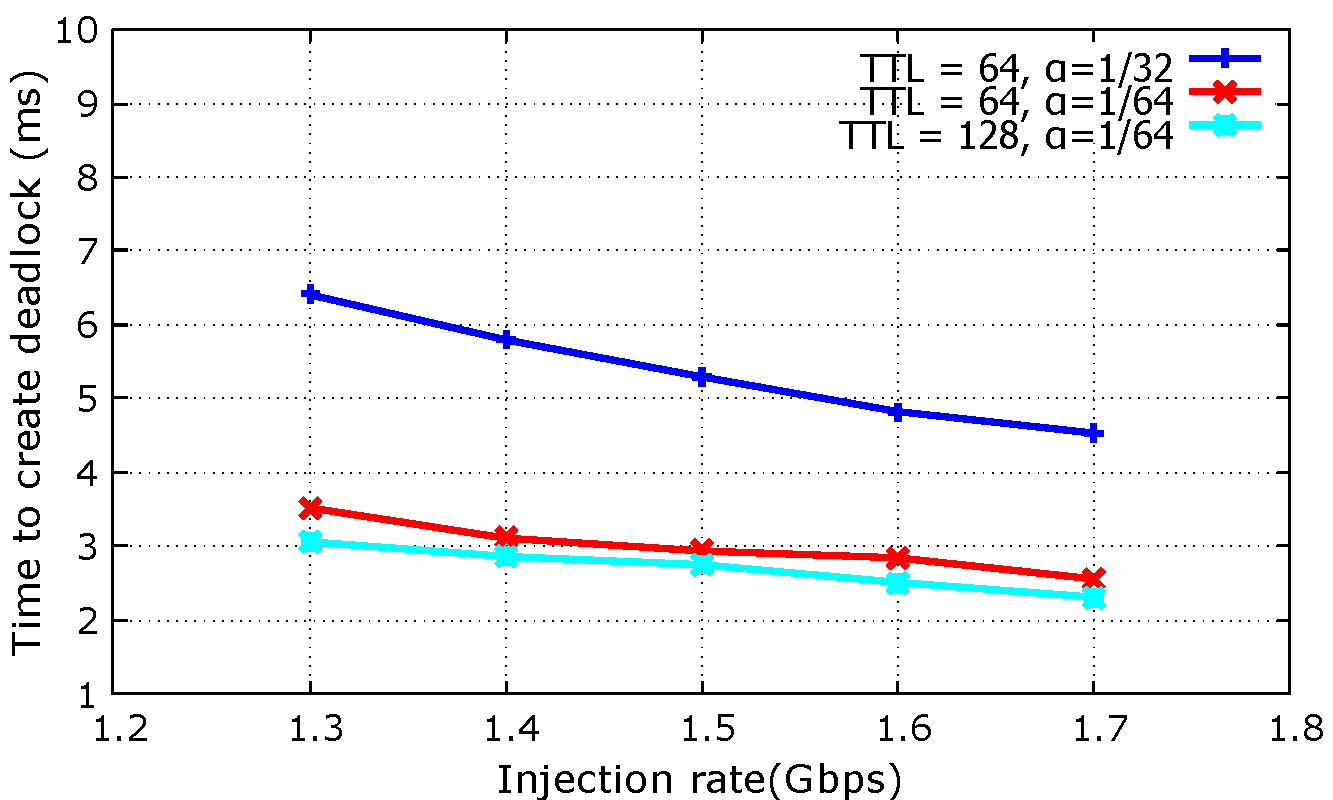
\includegraphics[width=0.5\textwidth,center]{figs/r_dltime.pdf}
\caption[Optional caption for list of figures]{Measurement of the time to create a deadlock under different settings (deadlock will not occur when the injection rate is less than 1.3Gbps).}
\label{fig:dltime_measurement}
\end{figure}

\parab{Measurement of the time to create a deadlock:} We manually configure a loop between two Arista 7050QX32 switches which have 32 full duplex 40Gbps ports and 12MB shared buffer. In Fig.~\ref{fig:dltime_measurement}, we set $\alpha$ and $TTL$ to different values and measure the time to create a deadlock under different injection rates.

We can make four observations from the results in Fig.~\ref{fig:dltime_measurement}: 1) It takes only a few milliseconds to create a deadlock even when the injection rate is less than 2Gbps. This indicates that it is easy for a deadlock to occur even when only a transilient loop exists in the network. In addition, we cannot rely on any loop detection and recovery solutions to prevent the occurance of deadlocks as they are too slow to resolve the loop within a few milliseconds. 2) As the injection rate increases, the time to create a deadlock decreases accordingly. 3) Given a fixed injection rate, a smaller $\alpha$ value requires less time to create a deadlock. 4) Given a fixed injection rate, a smaller TTL value requires more time to create a deadlock. This is because a smaller TTL value will make the packets get dropped faster in the loop, and thus more packets are needed to be injected into the loop to trigger switch to pause each other.

We repeated this experiment using many other combinations of TTL and $\alpha$ values and different number of switches. We found that all the results comply with what have been shown in Fig.~\ref{fig:dltime_measurement}.

The takeaway of this experiment is that: once there is a loop in the network, deadlock is easy to occur and very hard to prevent (a deadlock can be created within a few milliseconds). In addition to a fast loop detection mechanism, we need an effective solution to detect and resolve deadlocks caused by all kinds of loops.

%\parab{Estimation of the time to create a deadlock:} 

%\parab{Sufficient condition for deadlock creation:} \todo{(detailed content to be added later.)}
%
%   1. Analysis of the maximum packet drain rate caused by TTL expiration: $r^{max}_d = nB/k_ttl$.
%
%   2. Using testbed experiments to demonstrate that $r > r^{max}_d$ is a sufficient condition for deadlock creation.
%
%\parab{Creation time of deadlock:} \todo{(detailed content to be added later.)}
%
%   1. Analysis of the upper bound and lower-bound of the creation time of deadlock.
%
%   2. a) Using testbed experiments to demonstrate that lower-bound value is already a tight estimation when $r << B$; b) Analysis of the impact of PFC PAUSE frames on $r$ and $r^{max}_d$.
%
%\subsection{Analysis of device bug induced deadlock}\label{subsec:analysis_loop_deadlock}
%\todo{to be added.}